%%%%%%%%%%%%%%%%%%%%%%%%%%%%%%%%%%%%%%%%%%%%%%%%%%%%%%%%%%%%%%%%%%%%%%%%%%%%
% Formato en Látex para la generación de material de estudio en la ESPE - DECE 
% Documento generado en base a los formatos ejemplo otorgados por el Ing. Wilson Cerón
% Por:
% Dillan Aldás
% Andres Jimenez
% 
% Last Update: 2020.04.25 
%%%%%%%%%%%%%%%%%%%%%%%%%%%%%%%%%%%%%%%%%%%%%%%%%%%%%%%%%%%%%%%%%%%%%%%%
\documentclass[a4paper, 11pt]{article}
%Paquetes%%%%%%%%%%%%%%%%%%%%%%%%%%%%%%%%%%%%%%%%%%%%%%%%%%%%%%%%%%%%%%%%%%%
\usepackage[utf8]{inputenc}
\usepackage[T1]{fontenc}
\usepackage[spanish]{babel}
\usepackage{everypage}
\usepackage{graphicx}
\usepackage{lipsum}
\usepackage{tikz}
\usepackage{color}
\usepackage[left=3cm, right=2.75cm, top=4.5cm, bottom=4cm]{geometry}
\usepackage{fancyhdr}
\pagestyle{empty}
\usepackage{tikzpagenodes}
\usetikzlibrary{calc}
\usepackage{hyperref}
\usepackage{lipsum}
\usepackage[user,abspage]{zref}
\usepackage{siunitx}
\usepackage[square,numbers]{natbib}
\usepackage[maxbibnames=99, sorting=none, backend=bibtex]{biblatex}
\addbibresource{referencias.bib}
\usepackage{graphicx} 
\usepackage{spanish}
\usepackage{gensymb}
\usepackage{mathptmx}
\usepackage{amsmath}
\usepackage{calc}
\usepackage{latexsym}
\usepackage{amssymb}
%%Comandos y comandos nuevos %%%%%%%%%%%%%%%%%%%%%%%%%%%%%%%%%%%%%%%%%%%%%
%\newcommand{\slink}[2]{\hyperref[#1]{\underline{\smash{#2}}}} 
\renewcommand{\baselinestretch}{1.35} 

%% colores de los hyperlinks - 
% (en Adobe Acrobat los links Sí salen subrayados, en este visor de pdf solo salen azules) 
\hypersetup{%
colorlinks=true, linkcolor=blue, urlcolor=blue,linkbordercolor=blue, citecolor=blue, urlbordercolor=blue, pdfborderstyle={/S/U/W 1}
}
\makeatletter
\Hy@AtBeginDocument{%
  \def\@pdfborder{0 0 1}% Overrides border definition set with colorlinks=true
  \def\@pdfborderstyle{/S/U/W 1}% Overrides border style set with colorlinks=true
                                % Hyperlink border style will be underline of width 1pt
}
\makeatother
%colores%%%%%%%%%%%%%%%%%%%%%%%%%%%%%%%%%%%%%%%%%%%%%%
\definecolor{rojo_oscuro}{rgb}{.85,.45,.45} 
\definecolor{verde_oscuro}{rgb}{0,.5,.2} 
% Formato de todo el documento %%%%%%%%%%%%%%%%%%%%%
\AddEverypageHook{%
\tikz[remember picture,overlay]{%
% Páginas mayores a 2
  \ifnum\value{page}>1%
  % \ifnum\makeatletter\zref@extract{#1}{abspage}\makeatother>1%
  % \ifnum\value{\zref{abspage}}>1%
  % \ifnum\value{page}>1%
    \filldraw[fill=rojo_oscuro, thick,  draw=verde_oscuro] (1,-1.6) rectangle (16,-1.3);
    \filldraw[fill=rojo_oscuro, thick, draw=verde_oscuro] (1,-1.6-22.8) rectangle (16,-1.3-22.8);
        \node[anchor=east] at (16,-25) {\textcolor{black}{{\footnotesize DECE - ESPE}}};
        \node[anchor=west] at (1,-25) {\textcolor{black}{{\footnotesize \thepage}}};
  %logo DECE
        \node at (1.8,0) {\includegraphics[width=2.5cm]{DEEE_LOGO.png}};
%Pagina 1: Carátula%%%%%%%%%%%%%%%%%%%%%%%%%%%%%%%%%%%%%%%%%%%
  \else
    % Márgenes
    \filldraw[fill=rojo_oscuro, thick, draw=verde_oscuro] (-0.3,0) rectangle (0.3,-26); %izquierdo
    \filldraw[fill=rojo_oscuro, thick,  draw=verde_oscuro] (1,-1.6) rectangle (16,-1.3); %arriba
    \filldraw[fill=rojo_oscuro, thick, draw=verde_oscuro] (1,-1.6-21.8) rectangle (16,-1.3-21.8); %abajo
    % Texto de carátula
    \node[anchor=east] at (16,-24) {\textcolor{black}{{\Large Laboratorio de Circuitos eléctricos}}}; 
    \node[anchor=east] at (16,-25) {\textcolor{black}{{\small Procedimiento}}};
    \node[anchor=east] at (16,-25.8) {\textcolor{black}{{\footnotesize 2021}}};
    \node[anchor=east] at (16,-21) {\textcolor{black}{{\Huge Laboratorio 8}}};
    \node[anchor=east] at (16,-22) {\textcolor{black}{{\LARGE Teorema de la máxima transferencia de potencia}}};
    %Logos
    \node at (4.2,0.) {\includegraphics[width=6cm]{ESPE_LOGO.png}};
    \node at (14,0.) {\includegraphics[width=2.5cm]{DEEE_LOGO.png}};
 \fi}
 }
%
%
%
%
% \pagenumbering{roman}
%%%%%%%%%%%%%%%%%%%%%%%%%%%%%%%%%%%%%%%%%%%%%%%%%%%%%%%%%%%%%%%%%%%%%%%%%%%%%%%%%%%%%%%%%%%%%%%%%%%%%%%%%%%%%%%%%%%%%%%%%%%%%%%%
\begin{document}
\zlabel{iniciodedocumento}
\textbf{}
\newpage

\begin{flushright}
\textbf{\Huge Contenido}
\end{flushright}

\renewcommand*\contentsname{}
{% color de hyperlinks negro para el índice
\hypersetup{linkcolor=black, urlcolor=black,linkbordercolor=black, urlbordercolor=black, pdfborderstyle={/S/U/W 0.5}}
\tableofcontents
}



\newpage
%\pagenumbering{arabic} % empieza la numeración de página

\section{Procedimiento}

\begin{figure}[h]
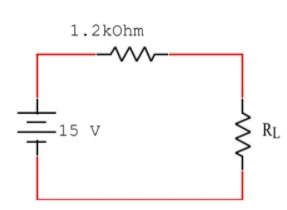
\includegraphics[scale=2.45]{CircuitoMTP.jpg}
\caption{Circuito para comprobar el Teorema de la Mtp}
\end{figure}

Para poder encontrar el voltaje en la resistencia variable $RL$ aplicamos un divisor de voltaje y a partir de ahí estructuramos una formula para que el cálculo sea mucho más sencillo y rápido, para este caso la formula quedaría de la siguiente manera:

\begin{equation*}
V_{RL}=\frac{RL}{RL+1.2K}*15
\end{equation*}

Para poder hallar la corriente en la resistencia $RL$ y evitar de llenarnos de cálculos podemos establecer una formula con la ayuda de la ley de ohm y como el circuito que estamos analizando es en serie la corriente será la misma para  todo el circuito entonces la formula es  la siguiente:

\begin{equation*}
I_{RL}=\frac{15}{RL+1200}
\end{equation*}

Para hallar la potencia consumida por la Resistencia aplicamos la siguiente formula

\begin{equation*}
P_{RL}=V_{RL}*I
\end{equation*}

Para $RL=220$

\begin{equation*}
V_{RL}=\frac{220}{RL+1.2K}*15=2.32V
\end{equation*}

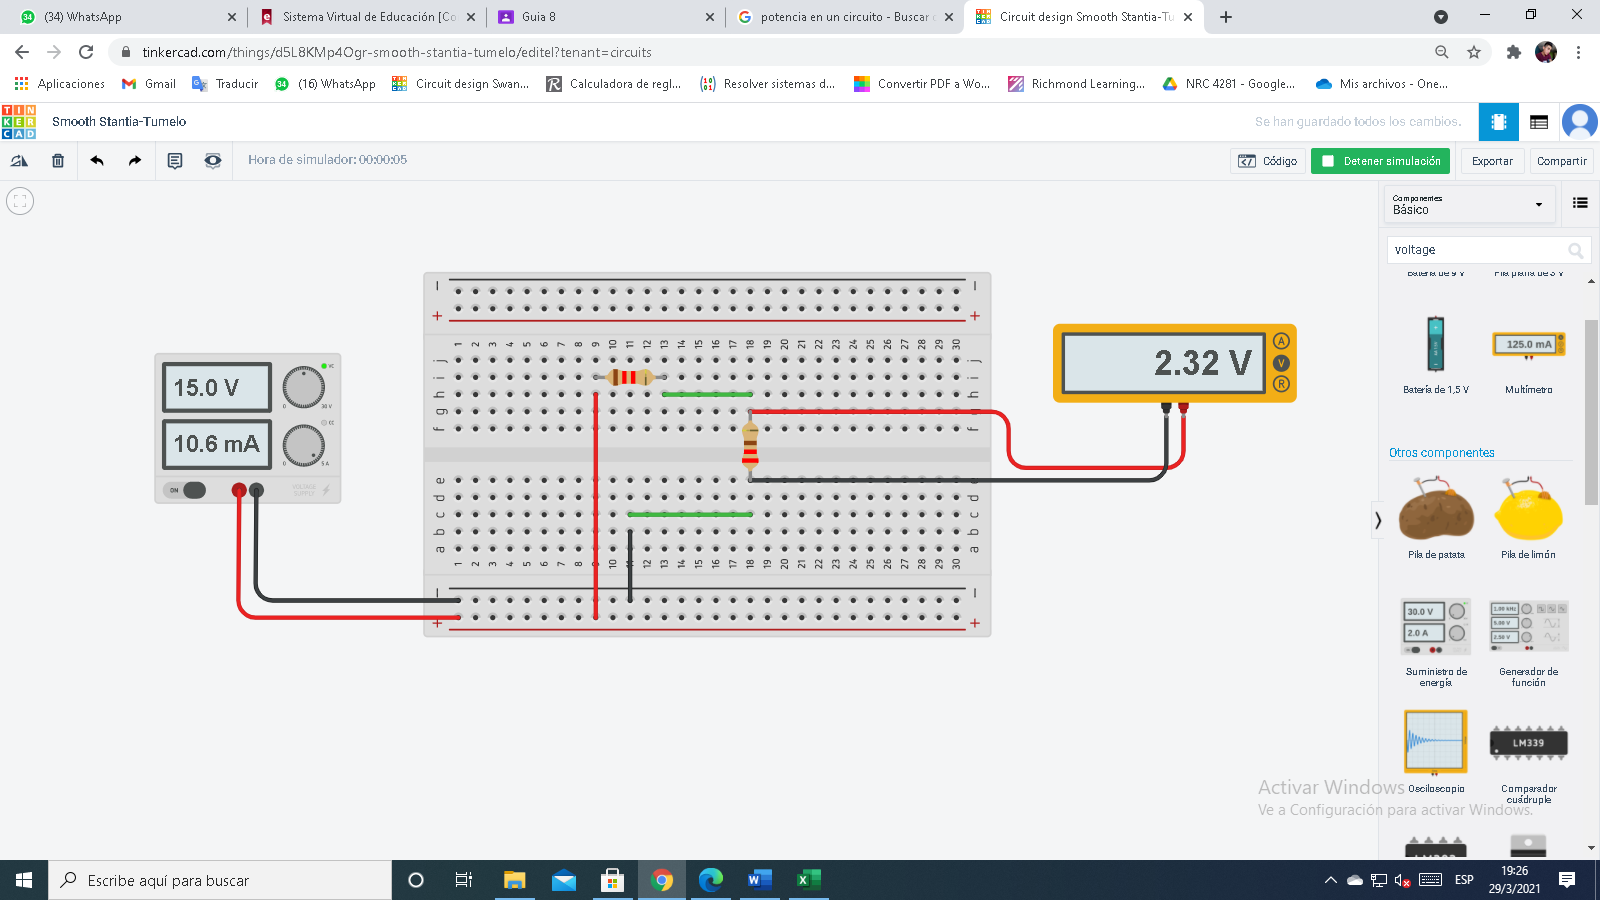
\includegraphics[scale=0.34]{V2020.png}

\begin{equation*}
I_{RL}=\frac{15}{RL+1200}=10.56mA
\end{equation*}

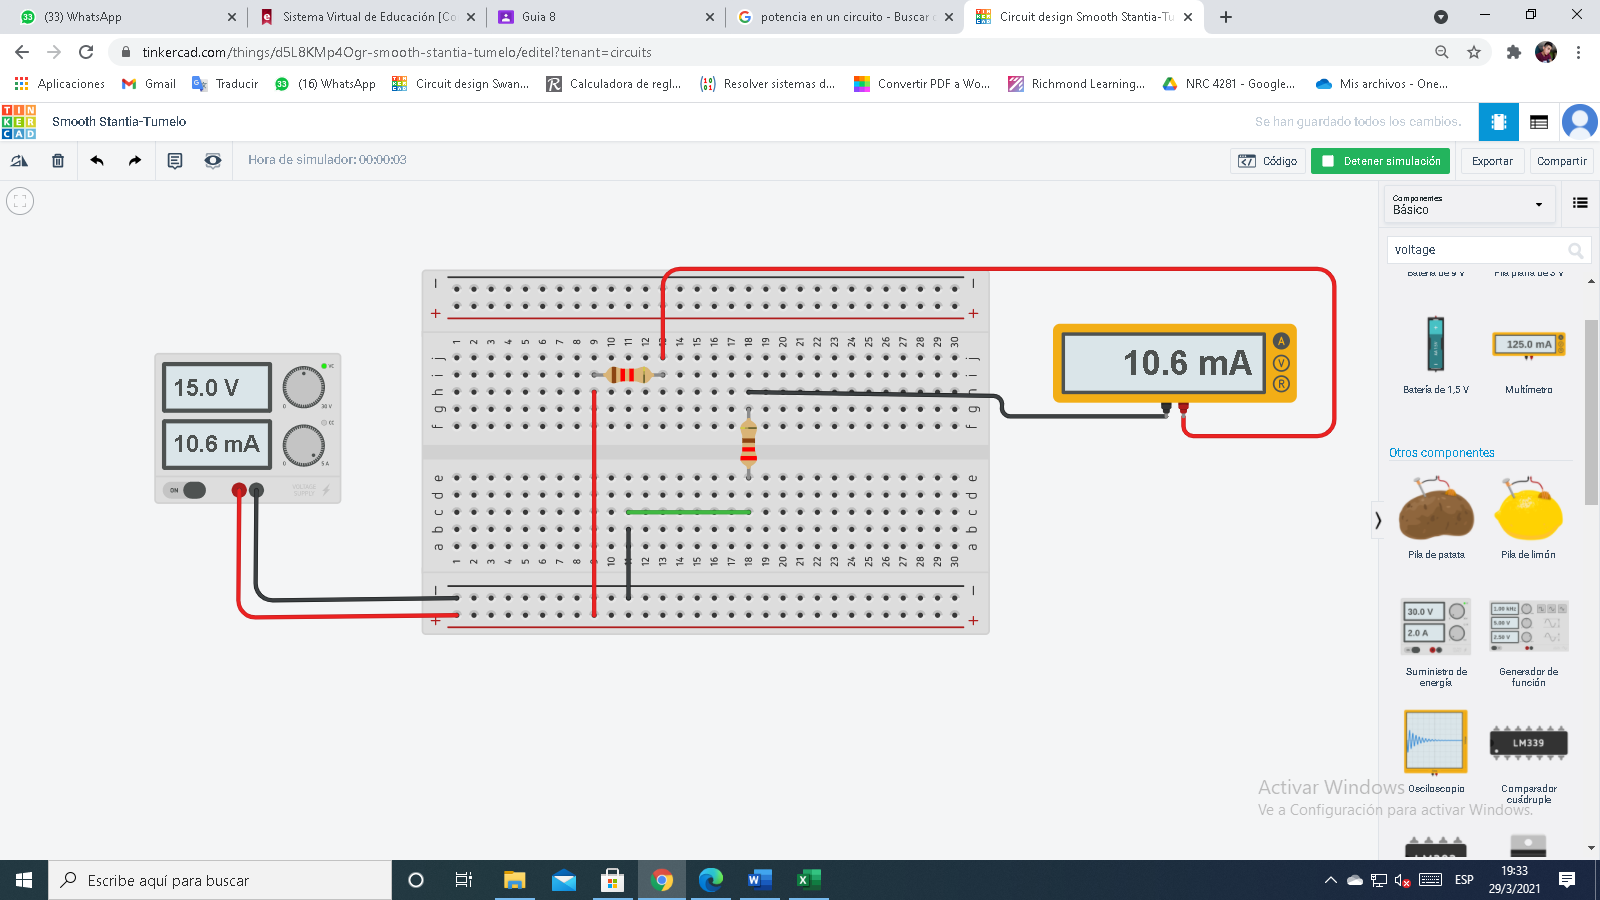
\includegraphics[scale=0.34]{I2020.png}

\begin{equation*}
P_{RL}=V_{RL}*I=2.32*10.56=0.024w
\end{equation*}

Para $RL=470$

\begin{equation*}
V_{RL}=\frac{470}{RL+1.2K}*15=4.222V
\end{equation*}

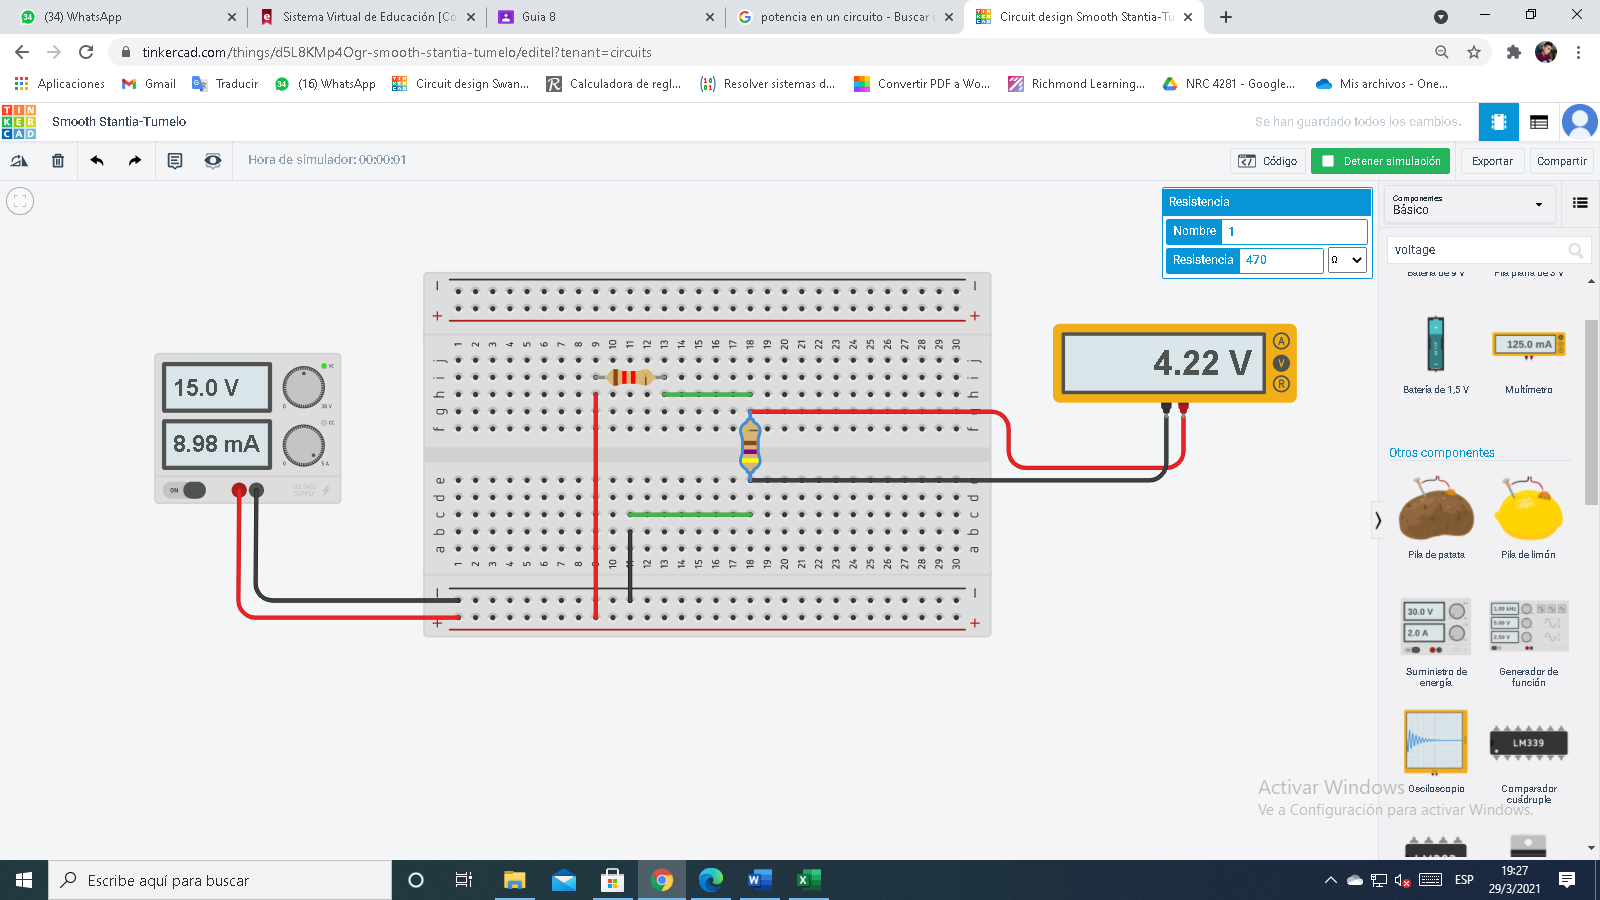
\includegraphics[scale=0.34]{V470.png}

\begin{equation*}
I_{RL}=\frac{15}{RL+1200}=8.9820mA
\end{equation*}

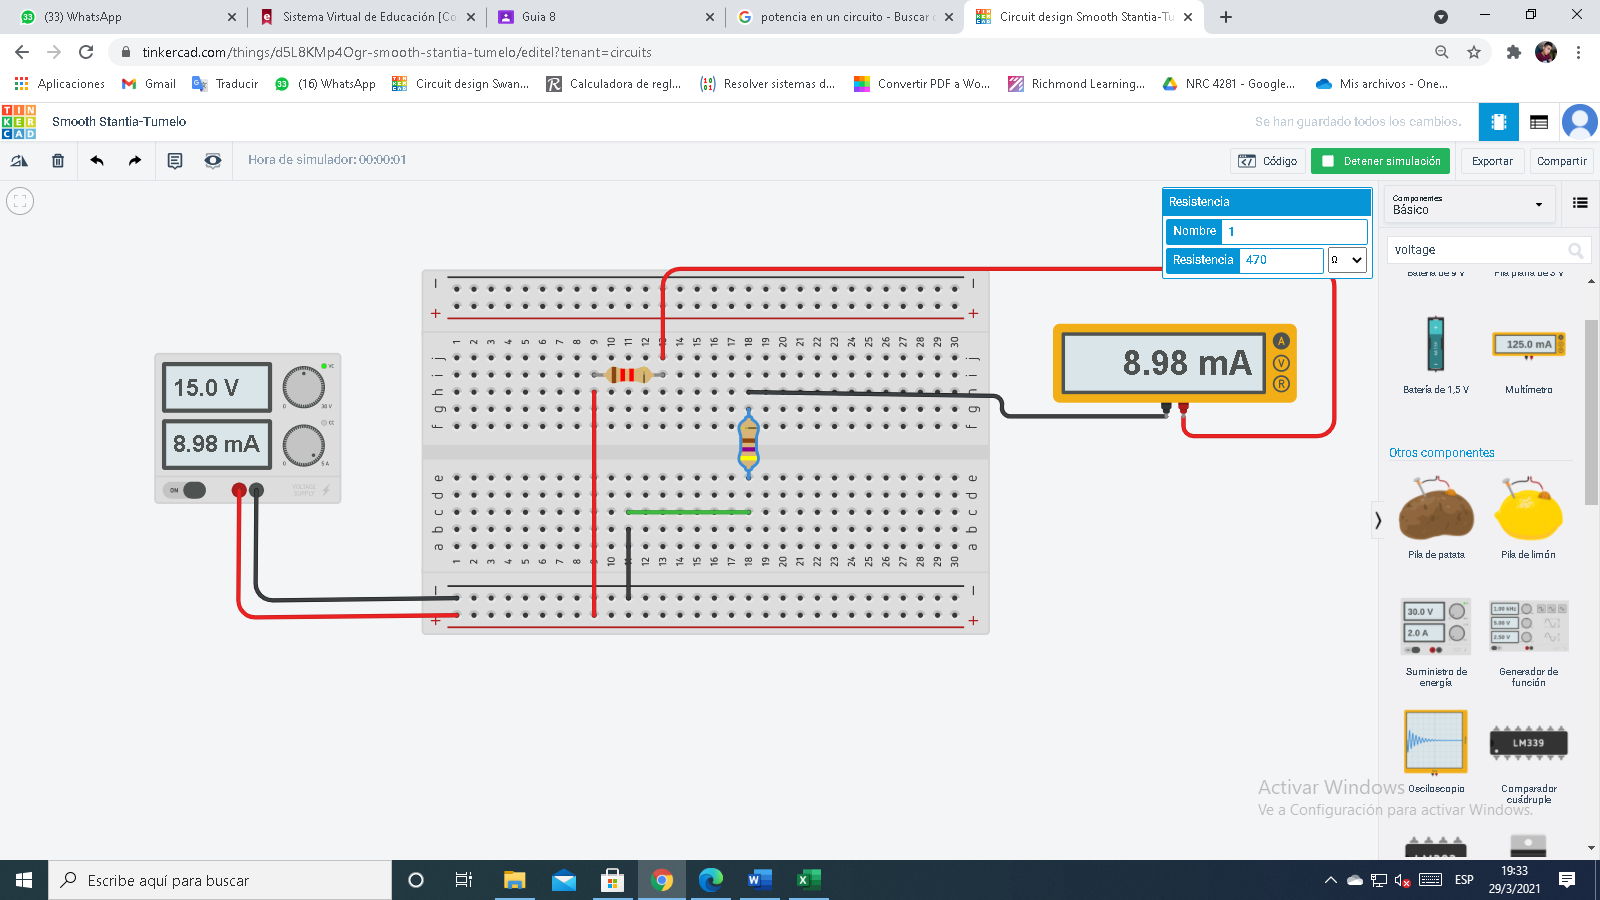
\includegraphics[scale=0.34]{I470.png}

\begin{equation*}
P_{RL}=V_{RL}*I=4.222*8.9820=0.03792w
\end{equation*}

Para $RL=680$

\begin{equation*}
V_{RL}=\frac{680}{RL+1.2K}*15=5.426V
\end{equation*}

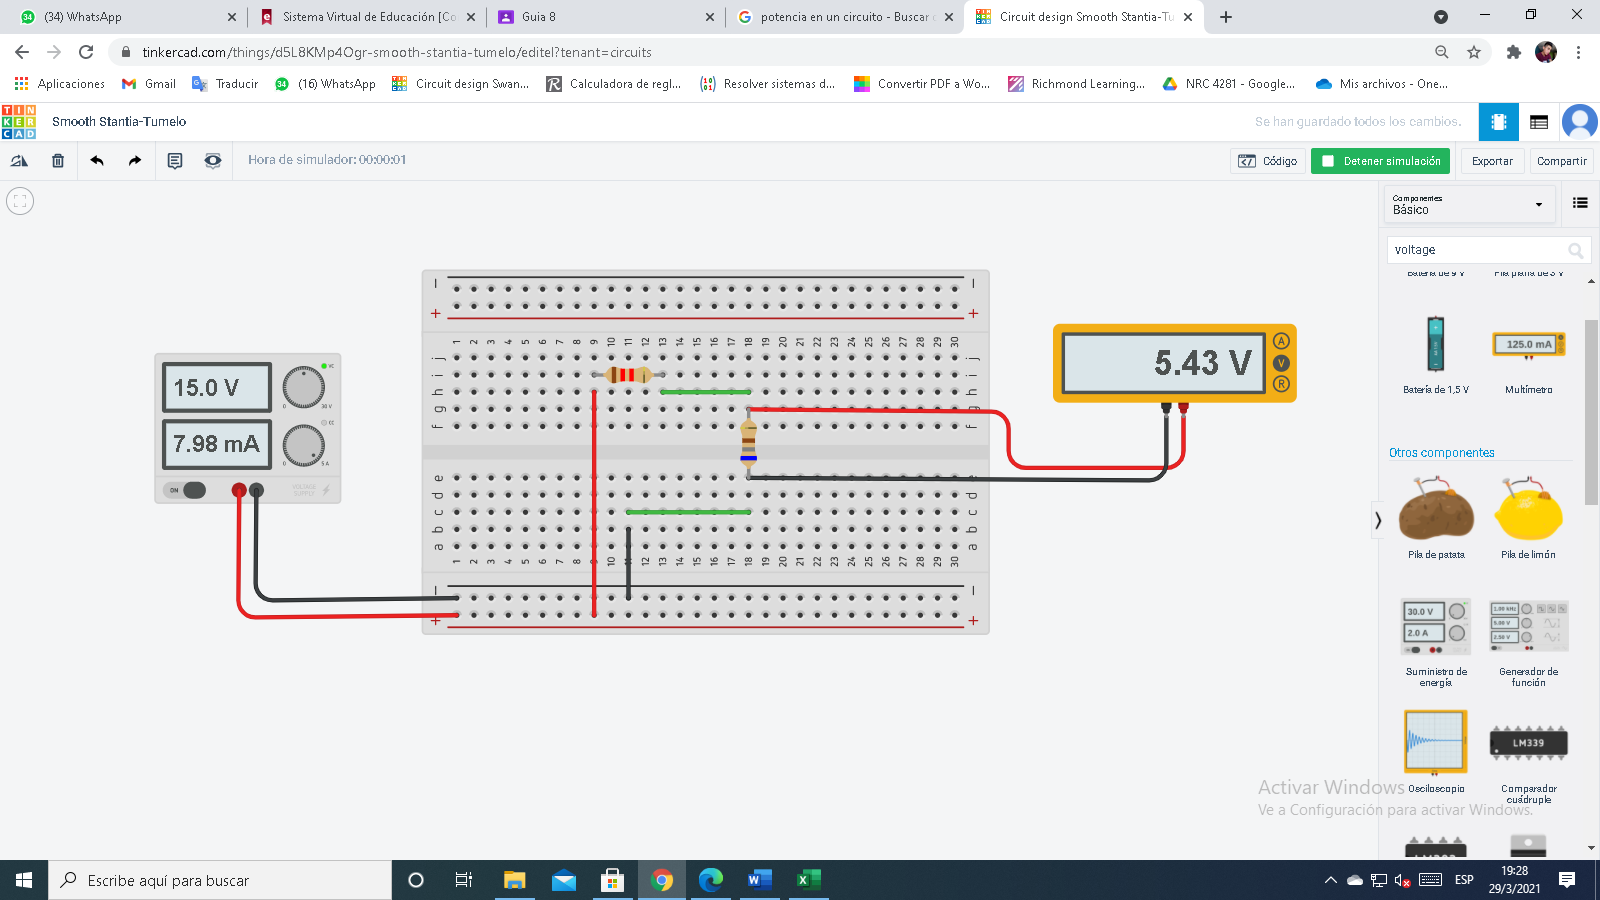
\includegraphics[scale=0.34]{V680.png}

\begin{equation*}
I_{RL}=\frac{15}{RL+1200}=7.9787mA
\end{equation*}

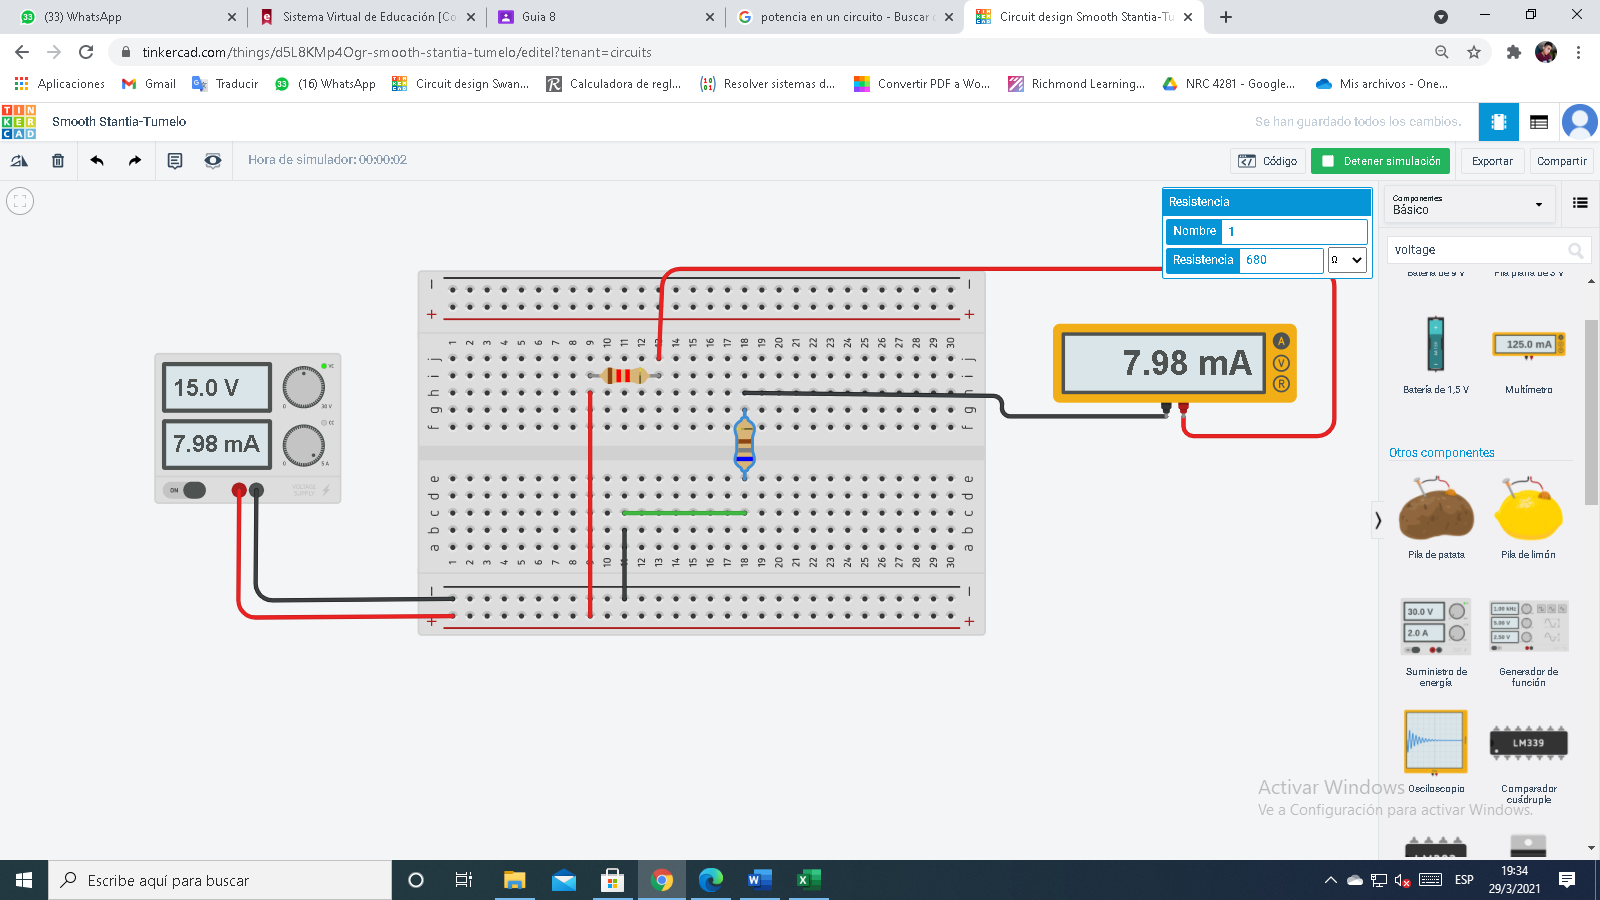
\includegraphics[scale=0.34]{I680.png}

\begin{equation*}
P_{RL}=V_{RL}*I=5.426*7.9787=0.04329w
\end{equation*}

Para $RL=820$

\begin{equation*}
V_{RL}=\frac{820}{RL+1.2K}*15=6.089V
\end{equation*}

\begin{equation*}
I_{RL}=\frac{15}{RL+1200}=7.4257mA
\end{equation*}

\begin{equation*}
P_{RL}=V_{RL}*I=6.089*7.4257=0.04522w
\end{equation*}

Para $RL=1k$

\begin{equation*}
V_{RL}=\frac{1000}{RL+1.2K}*15=6.818V
\end{equation*}

\begin{equation*}
I_{RL}=\frac{15}{RL+1200}=6.8182mA
\end{equation*}

\begin{equation*}
P_{RL}=V_{RL}*I=6.818*6.8182=0.04649w
\end{equation*}

Para $RL=1.5k$

\begin{equation*}
V_{RL}=\frac{1500}{RL+1.2K}*15=8.333V
\end{equation*}

\begin{equation*}
I_{RL}=\frac{15}{RL+1200}=5.5556mA
\end{equation*}

\begin{equation*}
P_{RL}=V_{RL}*I=8.333*5.5556=0.04630w
\end{equation*}

Para $RL=1.8k$

\begin{equation*}
V_{RL}=\frac{1800}{RL+1.2K}*15=9.000V
\end{equation*}

\begin{equation*}
I_{RL}=\frac{15}{RL+1200}=5.000mA
\end{equation*}

\begin{equation*}
P_{RL}=V_{RL}*I=9.0*5.0=0.04500w
\end{equation*}

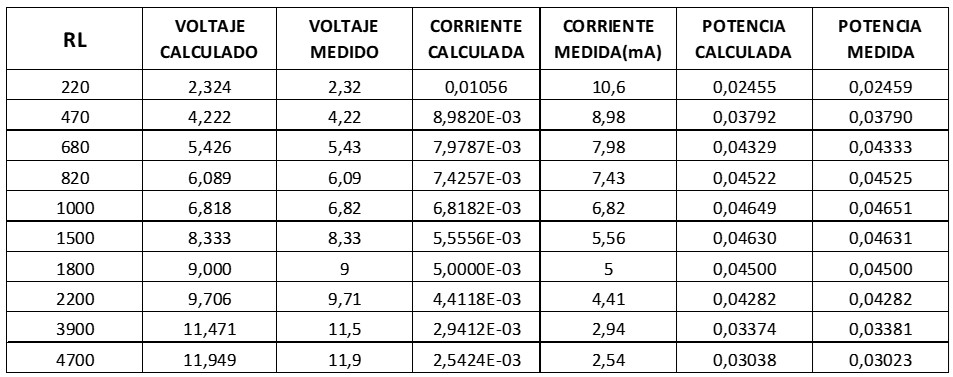
\includegraphics[scale=0.725]{TablaPotencia.jpg}

\end{document}